\documentclass[manuscript,review,anonymous]{acmart}
% \acmConference[]{} % need to include this to suppress addresses footer

\begin{document}

%\title{Design Patterns for Intelligent Musical Instruments: Case Studies in Performance with IMPSYpi}
% \title{Performing with Flexible and Accessible Intelligent Musical Instruments}
\title{Opening the Design Space: Performing with Intelligent Musical Instruments}

% Developing a Creative Practice with Intelligent Musical Instruments

\author{Charles Patrick Martin}
\email{charles.martin@anu.edu.au}
\orcid{0000-0001-5683-7529}
\affiliation{%
  \institution{The Australian National University}
  \city{Canberra}
  \state{ACT}
  \country{Australia}
}


\begin{abstract}
This paper is about making a cheap minimal battery-powered AI music controller, the GenAI MIDI Plug, that can be integrated into regular electronic music setups for exploring human-AI collaboration.
While machine generation of symbolic music and digital audio are hot topics there have been relatively few digital musical instruments that integrate generative AI, partly due to the complexity of training and deploying artist-centered generative AI systems.
This research introduces a minimal design for a generative AI controller based on an inexpensive single board computer that connects via MIDI to other musical devices.
Our approach uses a small artist-collected dataset that can be trained on a regular computer and very few hardware components.
This work demonstrates that real generative AI can occur on low-end hardware in an interactive music performance context. 
This system could be applied by a wide community of musicians and instrument designers to experiment with new intelligent musical instrument prototypes.
\end{abstract}

\keywords{generative AI, small data, human-AI interaction, intelligent musical instruments}

\begin{CCSXML}
<ccs2012>
   <concept>
       <concept_id>10010405.10010469.10010475</concept_id>
       <concept_desc>Applied computing~Sound and music computing</concept_desc>
       <concept_significance>500</concept_significance>
       </concept>
   <concept>
       <concept_id>10003120.10003121</concept_id>
       <concept_desc>Human-centered computing~Human computer interaction (HCI)</concept_desc>
       <concept_significance>500</concept_significance>
       </concept>
   <concept>
       <concept_id>10010147.10010257.10010293.10010294</concept_id>
       <concept_desc>Computing methodologies~Neural networks</concept_desc>
       <concept_significance>100</concept_significance>
       </concept>
 </ccs2012>
\end{CCSXML}

\ccsdesc[500]{Applied computing~Sound and music computing}
\ccsdesc[500]{Human-centered computing~Human computer interaction (HCI)}
\ccsdesc[100]{Computing methodologies~Neural networks}

\maketitle

\section{Introduction}\label{intro}

\begin{figure}
    \centering
    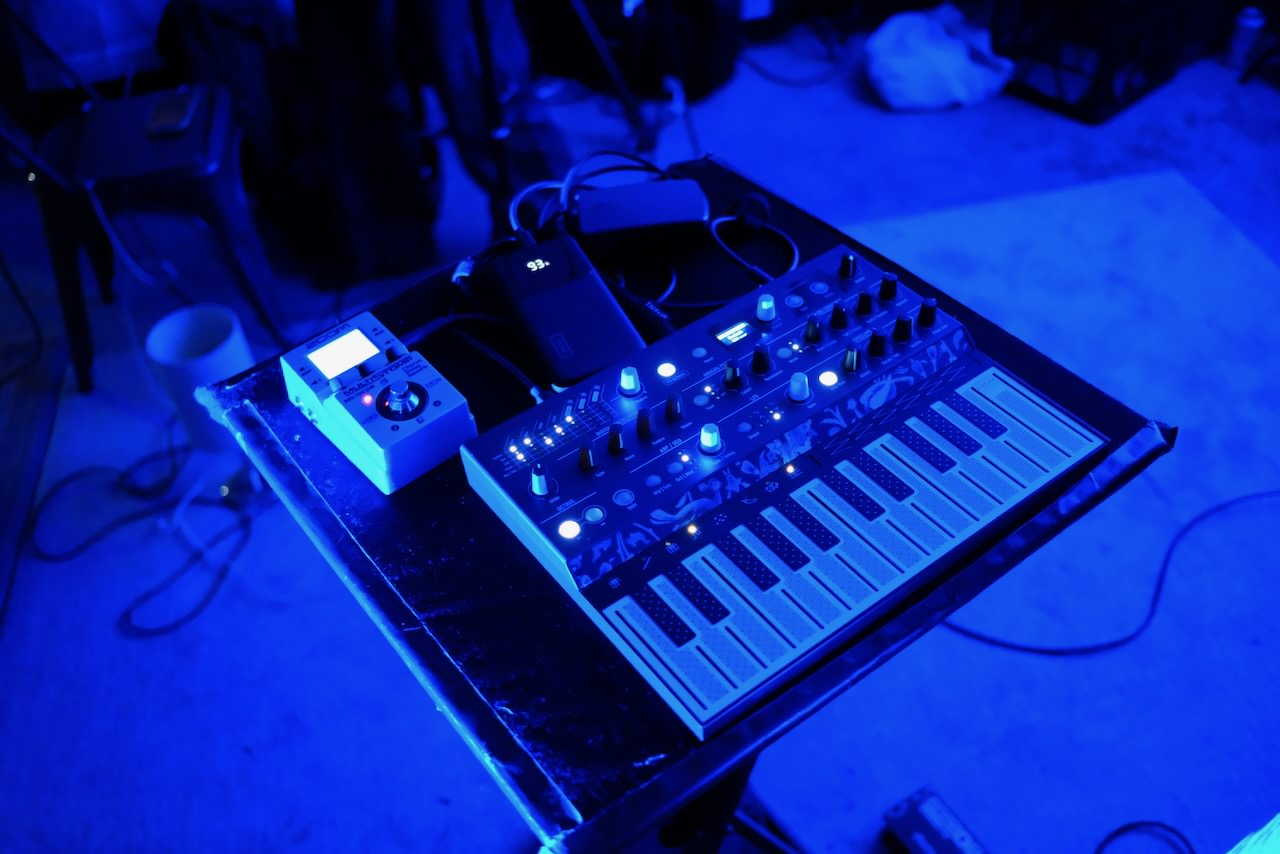
\includegraphics[width=0.8\linewidth]{figures/garage-concert-arturia.jpg}
    \caption{A battery-powered performance with an generative AI  synthesiser setup. Our software runs on the Raspberry Pi 4 which interacts with the synthesiser continuing and reacting to the musicians' actions.}
    \label{fig:enter-label}
\end{figure}

This paper explores how generative AI may be embedded within interactive musical systems for live performance through a series of case study instruments and performances where hardware and software synthesisers and instruments have been coupled with a Linux-based single board computer pre-loaded with generative AI software.
A broad range of music technology research has applied AI techniques, and in particular deep learning, for tasks such as mapping, audio or sensor analysis and musical data generation~\cite{jourdan_nime_ml_review}. 
While the analysis of gestures~\cite{visi_iml_gesture} remains a popular application, deep learning models now enable generation of audio~\cite{caillon_rave}, symbolic music~\cite{ji_survey_2024}, and interaction~\cite{Martin2019} data.
Despite this wide range of research, relatively few intelligent musical instruments, that is, digital musical instruments (DMIs) integrating generative AI, are available to be used in ordinary musical practice.
The goal of this research is to open the design space of intelligent musical instruments by introducing a system for creating these instruments that is cheap, small, battery-powered, thus enabling integration into a wider variety of musical systems by a diverse population of artists and experimenters. 
Our system includes AI software for generating expressive musical signals from small artist-centred datasets, runs on inexpensive Raspberry Pi computers, and is configurable via a web interface.
As an initial step towards identifying wider variety of intelligent musical instrument designs we report on series of instruments and performance experiences from a first-person perspective, illustrating different ways that this system can be incorporated into an artistic practice.

AI techniques have been applied in music performance at least since the 1990s with interactive systems such as Continuator~\cite{Pachet:2003wd} and Voyager~\cite{Lewis:2000fu} as well as tools such as Wekinator~\cite{fiebrink_meta-instrument_2009} for embedding machine learning models in new musical systems.
New and more capable deep learning techniques have led to an explosion of interest in AI music making at CHI workshops~\cite{genaichi2022}, music industry white-papers~\cite{goldmedia_ai_2024}, and the general media~\cite{musicpublishers}. Generative AI is now commonly frequently applied in tasks such as sound design~\cite{sound_design_ai_2024}, symbolic music generation~\cite{ji_survey_2024}, and music production~\cite{deruty_development_2022}; however, its use in live musical performances is less widely explored.
With many now framing generative AI as a threat to musicians' livelihoods~\cite{goldmedia_ai_2024} and fraught with ethical pitfalls~\cite{ethical_genaudio_2023}, it may be appropriate to introduce more artist-centred approaches to creating music with AI.

In this work we introduce a small-data~\cite{Vigliensoni:2022} approach to embedding AI within musical instruments where artists collect, curate, train, and deploy their own intelligent musical instruments.
We define an intelligent musical instrument as an instrument where an AI system generates actions independently of a musician's actions.
This definition would encompass Continuator~\cite{Pachet:2003wd} and Voyager~\cite{Lewis:2000fu} but exclude systems such as Wekinator~\cite{fiebrink_meta-instrument_2009} where AI is only used for mapping musicians actions.


% Our generative AI system includes an implementation of a mixture density recurrent neural network (MDRNN), appropriate for generating expressive musical signals from small artist-centered datasets. 
% This system can communicate to existing software and hardware musical systems using MIDI over USB, standard MIDI hardware connections, as well as OSC or WebSockets over a network.
% In this way, existing musical systems can be integrated with a generative AI system to create an intelligent musical instrument that can play by itself or take turns with and adapt to a human performer's input.
% In this research we introduce our generative AI system and explore its potential through a series of instrument designs and artistic research performances.
% Our experiments show that this idea is feasible and useful for experimenting with human-AI musical interaction.
% We distill lessons learned through ideation, development and performance with these systems to propose design recommendations for future intelligent musical instruments.
% This work could serve as a basis for prototyping further intelligent musical instruments and exploring their application in different creative practices.

Research applying generative AI on single board computers promises to allow these technologies to be embedded within self-contained musical instruments. 
This has been demonstrated for Raspberry Pi~\cite{Naess:2019aa, martin_empi} and Bela~\cite{pelinski_pipeline_bela} platforms. 
Previous work has acknowledged the difficulties faced by instruments builders wishing to embed AI within new instruments in terms of data collection and training~\cite{Martin2019} and cross-compiling code~\cite{pelinski_pipeline_bela}. These efforts are  mirrored in other creative design fields~\cite{teachablemachine}.
In contrast with very large and costly industrial-scale AI, these projects have emphasised a small data~\cite{Vigliensoni:2022} mindset where artists should collect, curate, train, and deploy their own AI systems. 

Framing a generative AI instrument as a MIDI plug leverages musicians' existing significant skills and understanding of their instruments which could allow a deeper co-creative practice with an AI system.
The present paper documents the process of creating our GenAI MIDI Plug showing that it is feasible, affordable and achievable for non-experts in AI. 
This process has also revealed pain points in setting up a generative AI instrument and new possibilities for co-creation that might encourage more widespread prototyping, hacking, and musicking with AI in NIMEs.

\section{Related Work}\label{related-work}

% This work reflects on previous research applying generative AI in performance, embedding AI within new musical instruments, and exploring new interfaces for musical expression through autoethnographic and artistic research methods. 

\subsection{Generative AI in Performance}

Martin et al.~\cite{martin_empi}

Jourdan and Caramiaux have identified gaps in interactivity and practice~\cite{jourdan_nime_ml_review} in AI-supported musical expression, particularly where deep learning is applied. 
They argued that as deep learning systems have become more complex there have been fewer examples of application in long-term musical practice and artists have less interaction with data collection and training phases. 
This contrasts with earlier parameter-mapping approaches where long term practice has been studied~\cite{fiebrink_years_ml}.
A small data approach to deep learning may only be part of the solution. 
It could be that engaging artists with simpler prototype systems that can be easily integrated into their existing practice could lead to more opportunities for data collection, training, and long-term practice.


\subsection{Embedded Musical Instruments}

Pelinski et al.~\cite{pelinski_pipeline_bela} demonstrated a pipeline for collecting data and training machine learning models for musical instruments built using the Bela embedded platform~\cite{mcpherson-bela-2016}.

Martin et al.~\cite{martin_empi} examined an embedded AI-based musical instrument and how different embodied representations of musical actions were perceived by improvisors.

\subsection{Research Methods}

This research explores generative AI instruments from a first-person or autoethnographic perspective~\cite{autoethnography-hci} where instruments are created and tested through autobiographical design~\cite{autobiographical-design}. 
This is related to the practice-based or -led approach~\cite{Smith:2009gf} often applied within creative arts research where knowledge is distilled from an artistic process. Artistic processes have been previously applied as sources of HCI knowledge~\cite{artistic-narratives-hci}. As the goal of this research is to expose design possibilities of a new system, it is appropriate to apply a first-person artistic perspective as an initial step.



\section{System Design}\label{sys-design}

Our generative AI interactive music system consists of Python software, a single board computer, a custom  operating system image that communicates to external electronic music devices over a USB, MIDI, or network connection. 
Unlike other embedded music systems, this setup is not intended to produce sound but only to control other electronic music devices so the single board computer does not need to have an audio output. 
Our system is designed so that a musician install the operating system image, which runs our software on boot, onto an SD card and configure the system from their computer using a web browser. 
After an initial setup the system can be incorporated into an electronic music setup for performances and experiments without further configuration. 
Alternatively, data recorded to the SD card can be retrieved and used to train new AI models for the system.
A diagram of our system in use is shown in Figure \ref{fig:system-diagram}.

\begin{figure}
    \centering
    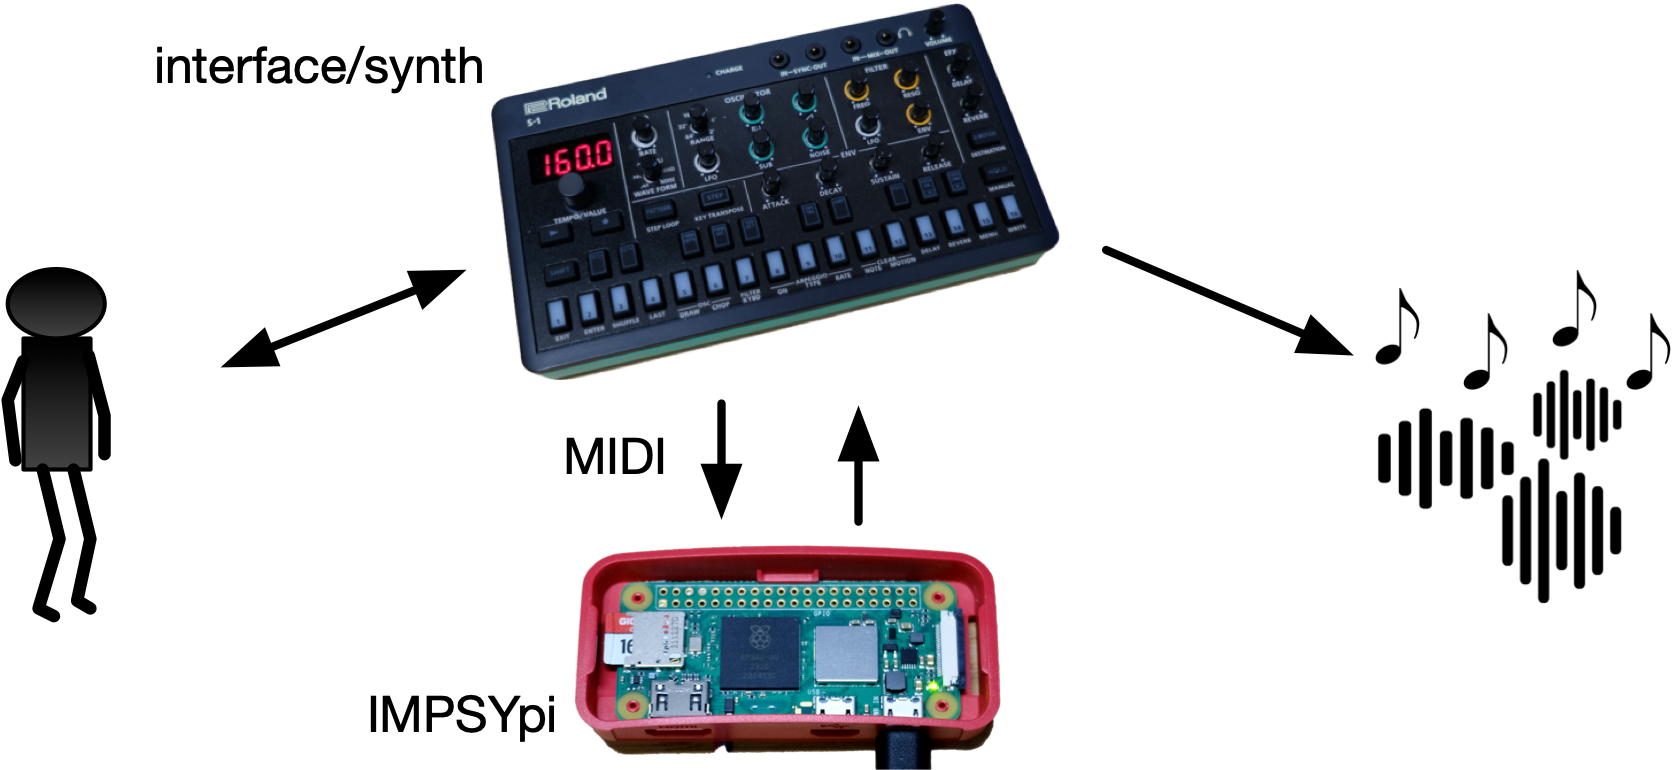
\includegraphics[width=0.8\linewidth]{figures/impsy-diagram.png}
    \caption{A diagram of our generative AI interactive music system with a hardware synthesiser and performer. Our system connects to other devices via MIDI and receives signals from a human performer or can send signals to control sound on the synthesiser. Our software is pre-installed on an operating system image for Raspberry Pi single board computers and runs on even the cheapest Raspberry Pi Zero 2 W (15USD).}
    \label{fig:system-diagram}
\end{figure}

\subsection{Hardware}

Our system uses the Raspberry Pi family of single board computers which are widely available and familiar for many electronic instrument designers. Our software works on all Raspberry Pi models that support the 64-bit Raspberry Pi OS which ensures good compatibility with machine libraries for Python. This includes the inexpensive Raspberry Pi Zero 2 W (15USD as of 2025) that includes a quad-core 64-bit ARM Cortex-A53 at 1GHz with 512MB of RAM and which is small enough (65mm x 30mm) to be incorporated inside new instrument designs or attached to existing instruments.

We have explored several methods of communicating with other devices from the Raspberry Pi. MIDI is used as the primary communication format and our software can send MIDI messages via either a USB-connected MIDI interface, a direct USB MIDI connection to a hardware synthesiser, or from the Raspberry Pi's serial (UART) output. Our software can also communicate over a network using OSC (open sound control) or WebSockets messages. The smallest Raspberry Pi Zero models only support one USB host connection while larger models (e.g., Rasberry Pi 4 Model B) have multiple USB host ports and an Ethernet interface so could support multiple communications channels simultaneously.
For MIDI-over-serial connections, the MIDI connector can be soldered to the GPIO pads corresponding to the Pi's serial (UART) output. 
Providing a MIDI output from the Pi's 3.3V signals is straightforward requiring only two resistors~\cite{MIDI-Manufacturers-Association:2014aa}: 10$\Omega$ between the UART TX pin and pin 5 on the MIDI connector and 33$\Omega$ between the 3.3V output and MIDI pin 4. 
MIDI pin 2 is connected to ground. 
In the setup shown in Figure \ref{fig:self-playing-volca}, the resistors are concealed within the MIDI connector.

% \begin{figure}
%     \centering
%     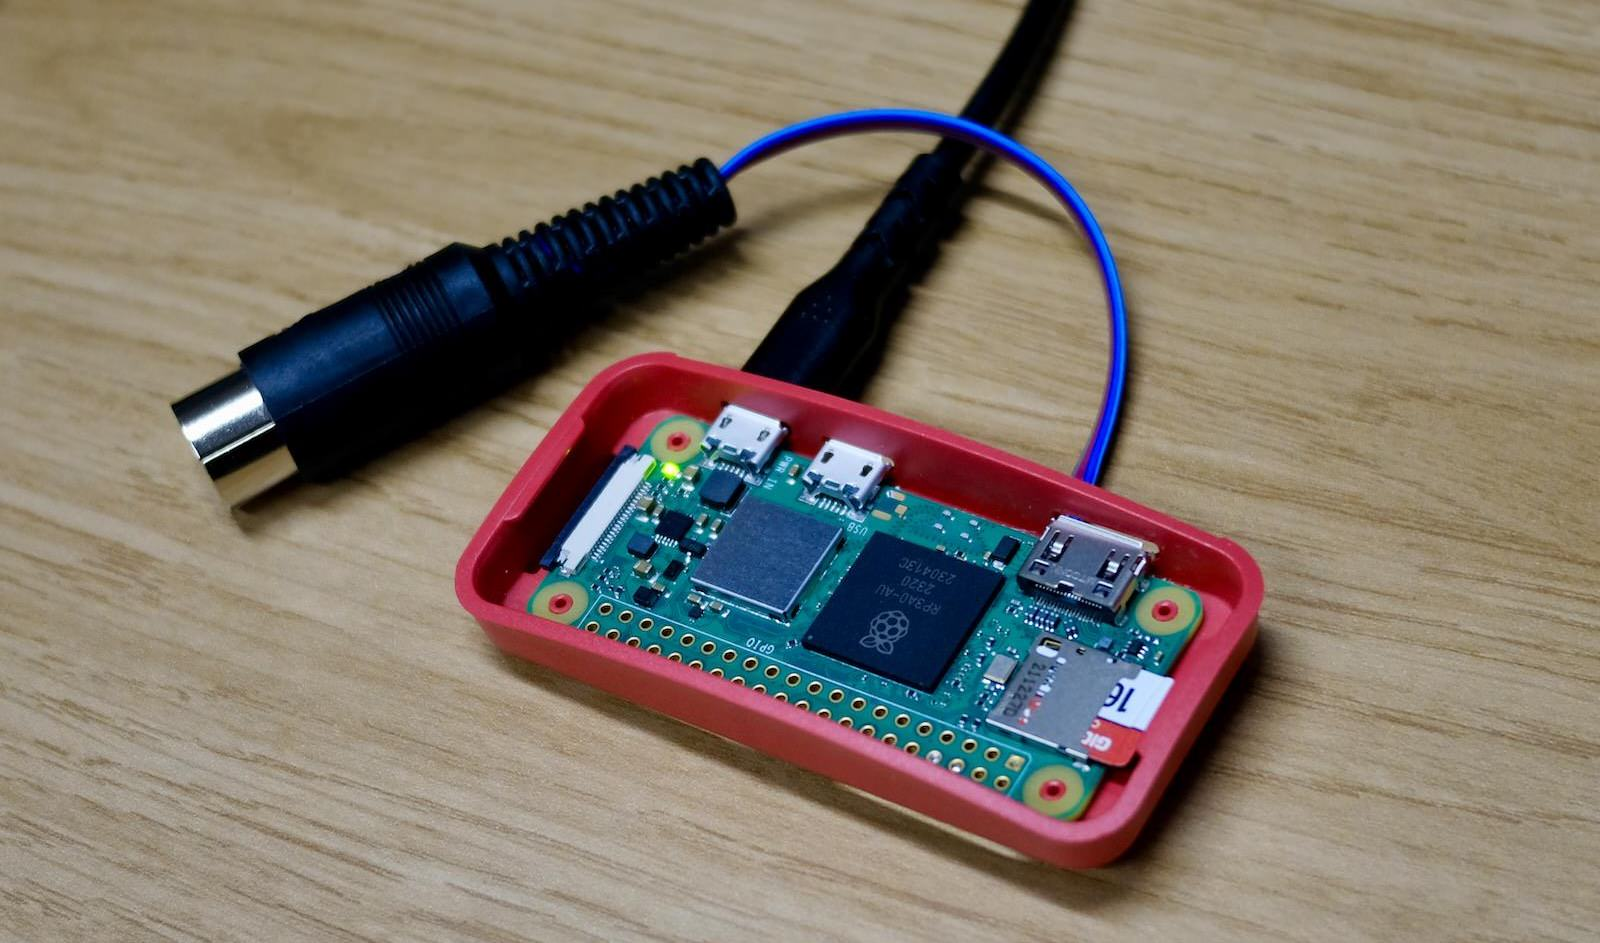
\includegraphics[width=0.8\linewidth]{figures/desk-angle.jpg}
%     \caption{The GenAI MIDI Plug with cover removed. The hardware consists of a Raspberry Pi Zero 2 W with case, 16GB microSD card, and a MIDI connector soldered directly to the Raspberry Pi.}
%     \label{fig:system-photo}
% \end{figure}

\subsection{AI model}

Following Martin and Torresen~\cite{Martin2019}, we use a mixture density recurrent neural network (MDRNN) as the machine learning paradigm for generating a stream of musical data and we apply the Keras-MDN-Layer library~\cite{keras-mdn-layer} to construct this neural network.
Our system uses an MDRNN that generates tuples of data that we interpret as number of musical values and a time delta for when that value should occur in the future. 
The number of musical values is configurable within our software but is at a minimum one, i.e., the system models one musical parameter over time, and we have experimented with up to 16 parameters modelled simultaneously.
The neural network is autoregressive, so takes the preceding value as input to the generate next, but it is also recurrent, so it stores a lossy history of generated values using LSTM units. 
We typically use small MDRNN models, e.g., 2 layers of 64 LSTM units.
Although this is a very small number of parameters compared to industrial generative AI and large language models, it is sufficient for generating musically useful data in real-time on small hardware.

Full evaluation of this AI model is beyond the scope of this paper, but we have benchmarked the inference speed. Our experiments showed that with the small models we use (2-layer LSTM with up to 256 units) individual inference steps are completed in under 5ms on all compatible Raspberry Pis (Zero 2 W, 3 Model B, 4 Model B) and well under 1ms on the Raspberry Pi 5. These inference speeds are sufficient for representing smooth MIDI signals. The time for training a new model depends on the size of the training data and speed of the training computer, but effective models can be trained in under 30 minutes on a normal laptop.

% \begin{figure}
%     \centering
%     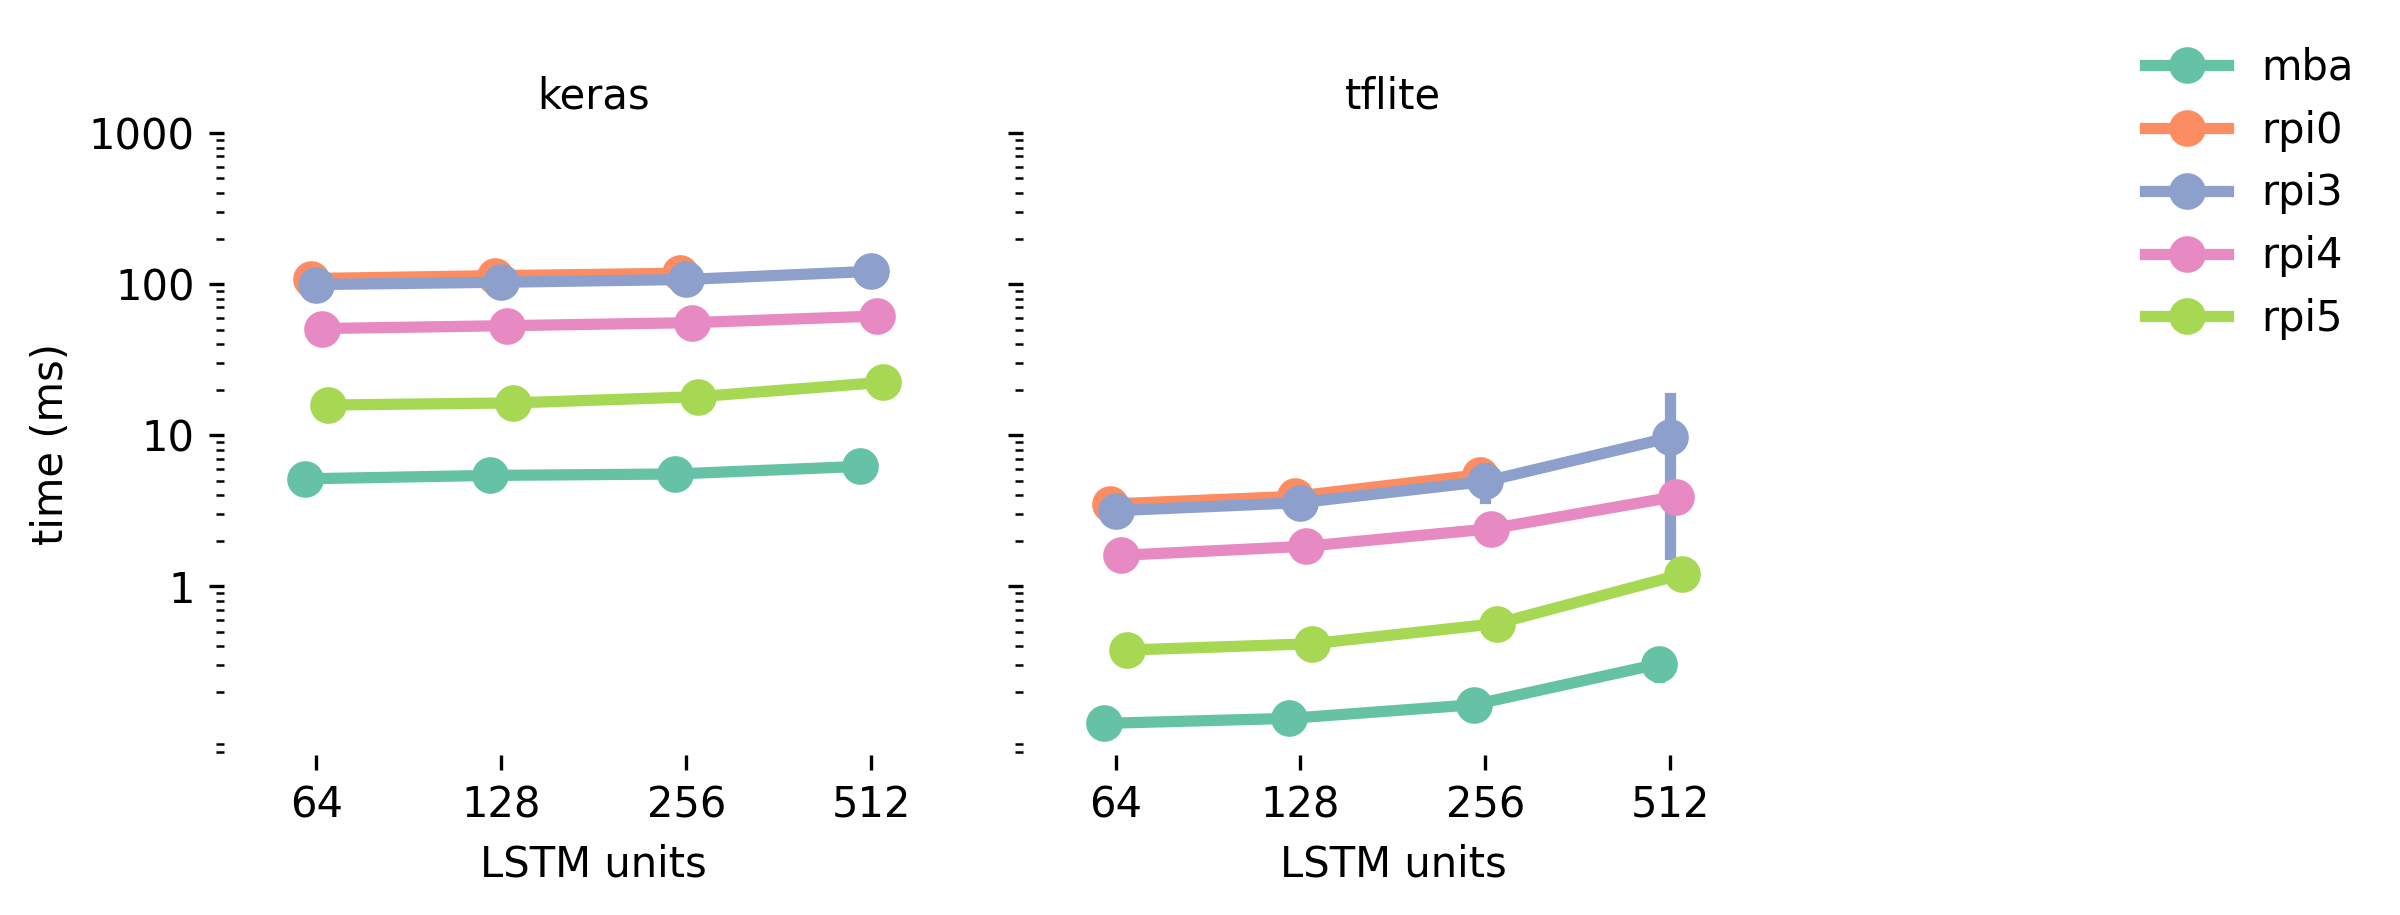
\includegraphics[width=0.99\linewidth]{figures/prediction_time_against_units_facet_log.png}
%     \caption{A plot of the time for single AI predictions on different hardware and model size. Even the slowest Raspberry Pi Zero 2 W runs predictions under 5ms using Tensorflow Lite.}
%     \label{fig:inference-time}
% \end{figure}

\subsection{Software}

Our system's software is a Python program running on the Raspberry Pi that generates musical data and sends it to external electronic musical instruments.
This program listens to MIDI signals from the instrument and responds with AI-generated continuations of the performance state.
MIDI note-on as well as control change messages are supported so our system is able to play notes as well as change the timbre of a connected instrument.
As mentioned above, our AI model is capable of listening and responding to a number of channels of such MIDI data simultaneously.
Our software records all data that is received from the MIDI interface and stores this as timestamped logs. This means that performing with our system builds up new datasets allowing new AI models to be trained.

An initial configuration is required to choose the MIDI interface and the specific MIDI signals listen and send to. 
Configuring such interaction mappings is a design task that fundamentally changes how a created intelligent musical instrument will function. 
For example, it may be interesting only assign timbral changes to the generative AI system while a performer controls notes (or vice-versa). Alternatively, the performer's notes can be cross-mapped to influence the timbral parameters changed by the generative AI system.
A simple web interface is provided for adjusting the configuration file, downloading logged data of previous performances and uploading new AI models.

The software for our system is distributed can be installed using Poetry but this can be a laborious process for new users. 
To accelerate setup with a new instrument we pre-install our software on a Raspberry Pi OS image that can be flashed to an SD card. 
Our OS image automatically starts the generative AI interaction system and web server programs as and also enables Ethernet-over-USB so that the Raspberry Pi can be directly connected to a computer for configuration.



\section{Performance Experiences}\label{case-studies}

This section describes a series of musical performances where the author used IMPSYpi to create intelligent musical instruments and performed with them in live concerts.
We have applied an exploratory and autobiographical artistic research approach where these instruments have been developed for our own use and tested in authentic live performance situations.

\subsection{The Self-Playing Volca}

% \begin{figure}
%     \centering
%     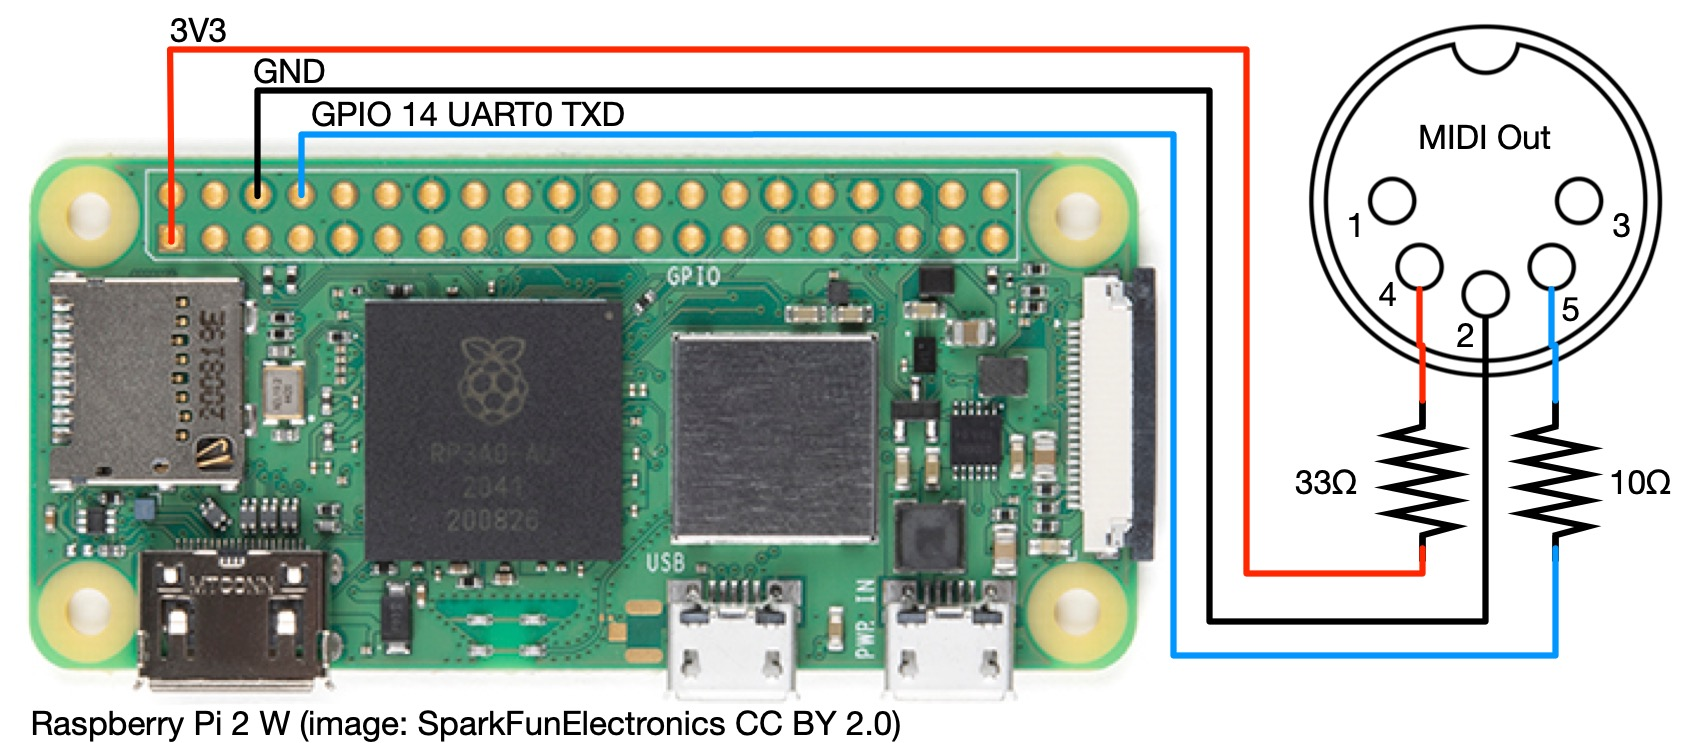
\includegraphics[width=\columnwidth]{figures/sf-image.jpg}
%     \caption{Circuit diagram for the GenAI MIDI Plug. A MIDI output can be obtained from a Raspberry Pi with the addition of only two resistors that can be concealed inside the MIDI connector.}
%     \label{fig:enter-label}
% \end{figure}

\begin{figure}
    \centering
    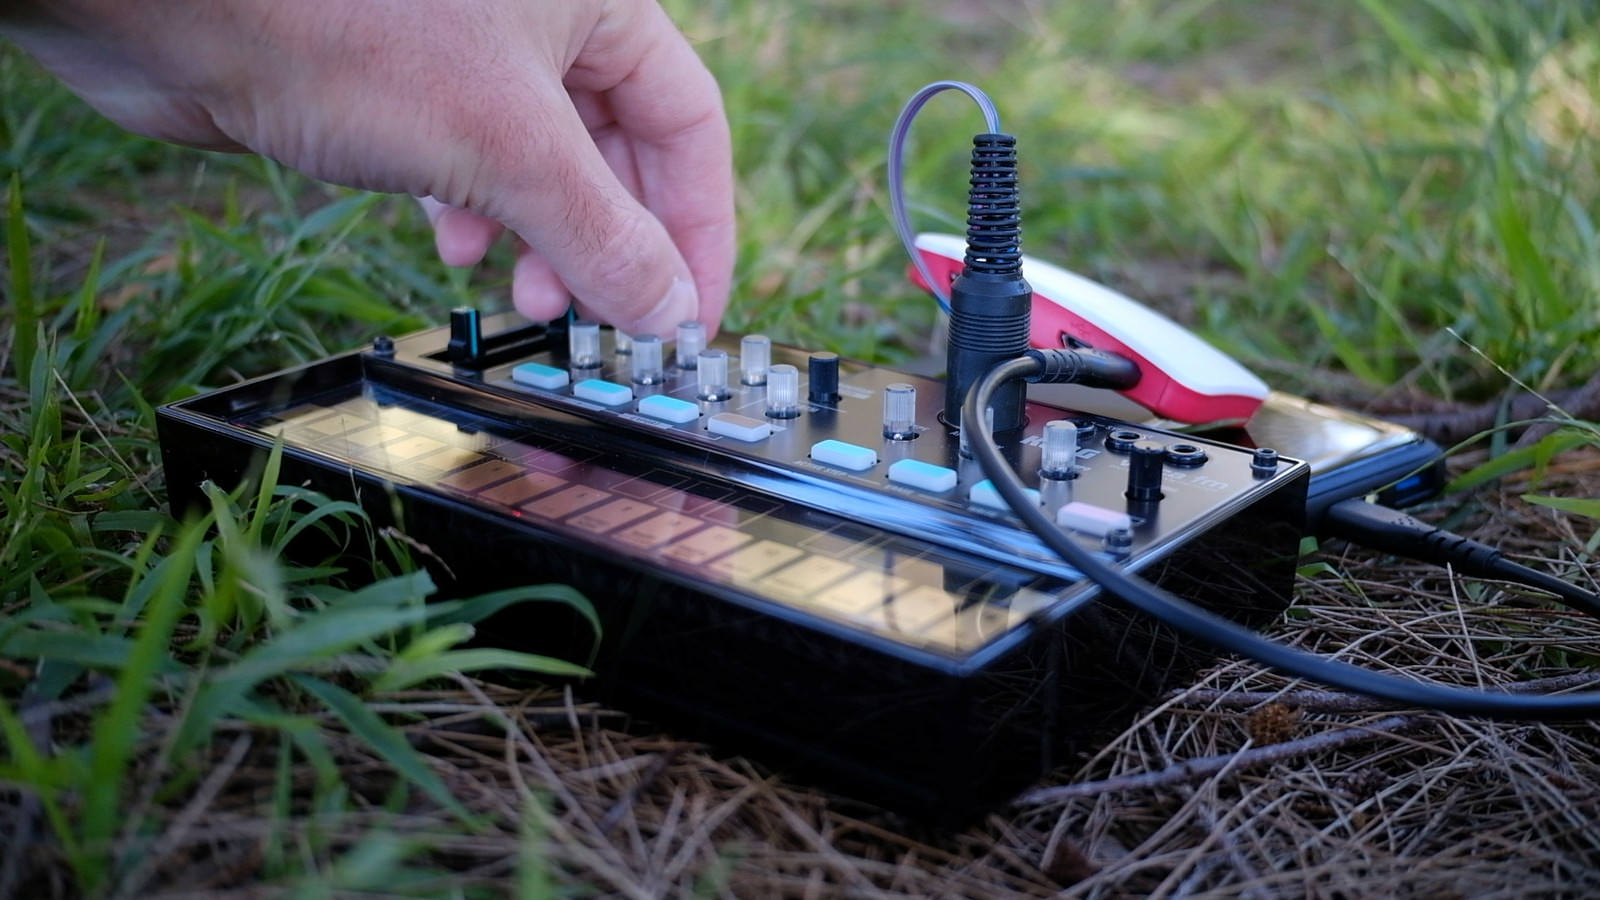
\includegraphics[width=0.8\linewidth]{figures/outside-1.jpg}
    \caption{Battery-powered human-AI interaction on a Korg Volca FM. The generative AI system running on the Raspberry Pi Zero controls pitch and rhythm via the MIDI connector while the musician edits the synth patch. 
    % Video: \url{https://vimeo.com/911078203}
    }
    \label{fig:self-playing-volca}
\end{figure}

The self-playing Volca was a proof-of-concept design to establish whether real-time generative-AI MIDI signals from the Raspberry Pi Zero was feasible and musically interesting.
For this design, a simple MIDI output was obtained from the Raspberry Pi's GPIO header UART pins.
The output was connected to the battery-powered Volca FM and the Raspberry Pi itself was powered by a USB power bank.
Initially, only pitch and rhythm was controlled by the IMPSYpi.
The MDRNN was trained on a corpus of 65 minutes of musical human interaction with a single continuous controller. This corresponded to around 75000 interaction events (value and time delta).
The corpus consisted of data with continuously changing values between 0 and 1 and time deltas recorded in seconds. This is somewhat different to melodic MIDI note data that is often used in musical AI. 
The MDRNN output (0.0--1.0) was converted to a MIDI pitch value from 0--127 and a corresponding MIDI note-on message scheduled to be sent at the time-delta generated by the MDRNN.

This initial experiment emphasised portability with a completely self-contained and battery-powered system: the Volca FM even has an internal speaker.
While the MDRNN could play notes, and a human performer could adjust the synthesiser's timbre or settings as well as play overlapping notes on the keyboard, the MDRNN couldn't respond to the performer as the Volca FM does not have a MIDI output.
This meant that although this experiment started to explore different roles for the human and MDRNN in controlling the synth, the interaction was necessarily one way.

This experiment also showed that musical performance of the MDRNN when transformed to MIDI note-on commands is quite different from other generative AI MIDI performance systems. Traditionally , AI MIDI systems are trained on compositions or melodies, while this system was trained on expressive interaction with a continuous controlled. 
The resulting performances are include glissandi of various speeds, starting points, and lengths.
Sent through the Volca FM, these can sound unusual as the synthesiser retriggers it's envelope for each note.
This dataset may be more applicable to synthesis parameter control tasks where a musician would like a particular value to change smoothly in an expressive way including varying speed and pauses.


\subsection{The Intelligent MicroFreak}

\begin{figure}
	\centering
	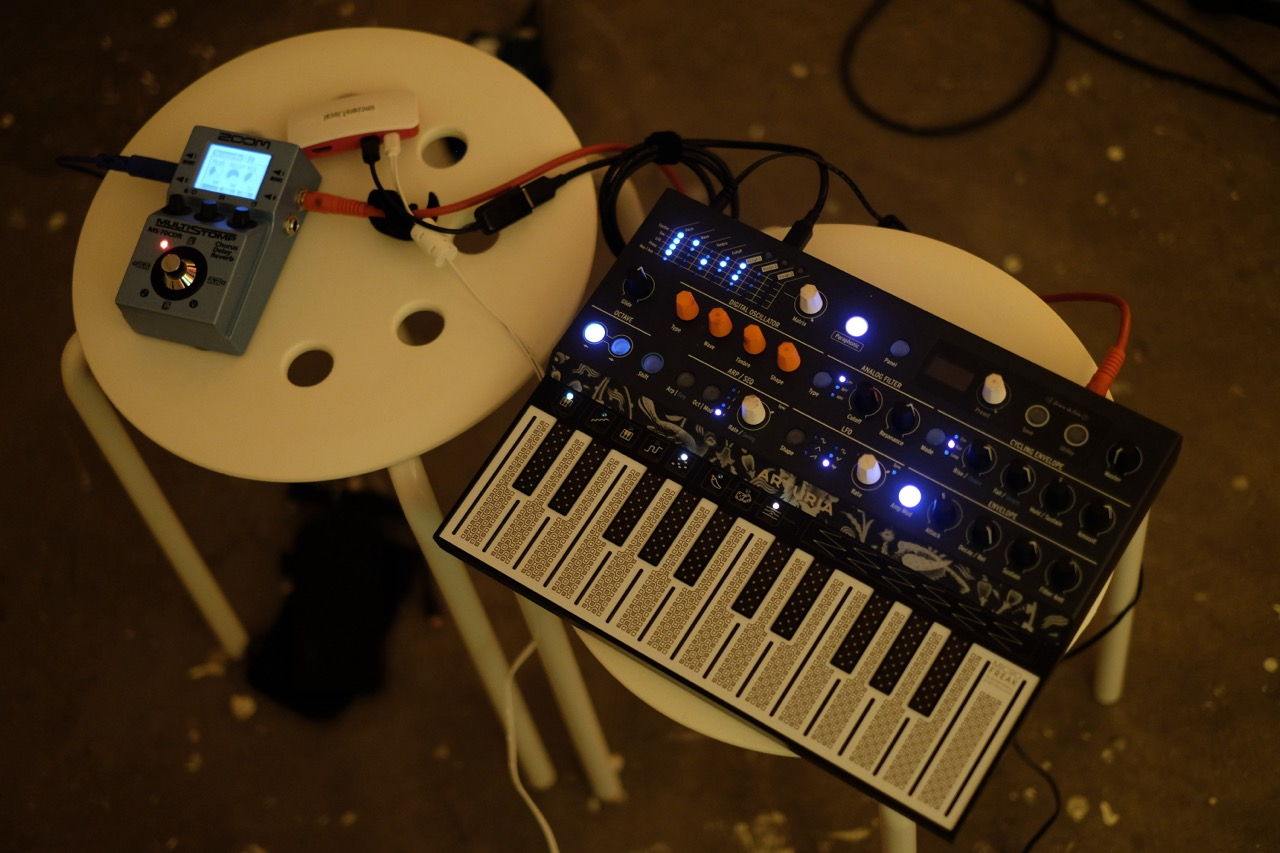
\includegraphics[width=0.8\linewidth]{figures/intelligent-microfreak.jpg}
	\caption{The intelligent MicroFreak setup on stage. IMPSYpi runs on a Raspberry Pi Zero 2 W (upper left), the Arturia Microfreak (lower right) is the main instrument while a Zoom effects pedal (lower left) provides additional audio effects.}
	\label{fig:microfreak}
\end{figure}


While the above example demonstrated one-way input from IMPSYpi into a hardware synthesiser, other systems promised to support two-way interaction. 
Establishing a MIDI-over-USB connection between IMPSYpi and a hardware synth often allows physical controls on the synthesiser to send signals to the IMPSYpi while simultaneously controlling the synthesiser.
The IMPSYpi is then configured to behave in a call-and-response manner so that when the human is adjusting the synth controls and playing notes, these IMPSYpi tracks these signals and only when the human stops for a certain amount of time does the IMPSYpi take over the controls. 
This arrangement was first trialled with an Arturia MicroFreak synthesiser with IMPSYpi controlling 8 parameters: note-on messages

\subsection{Performing with others: Intelligent S-1}

\begin{figure}
	\centering
	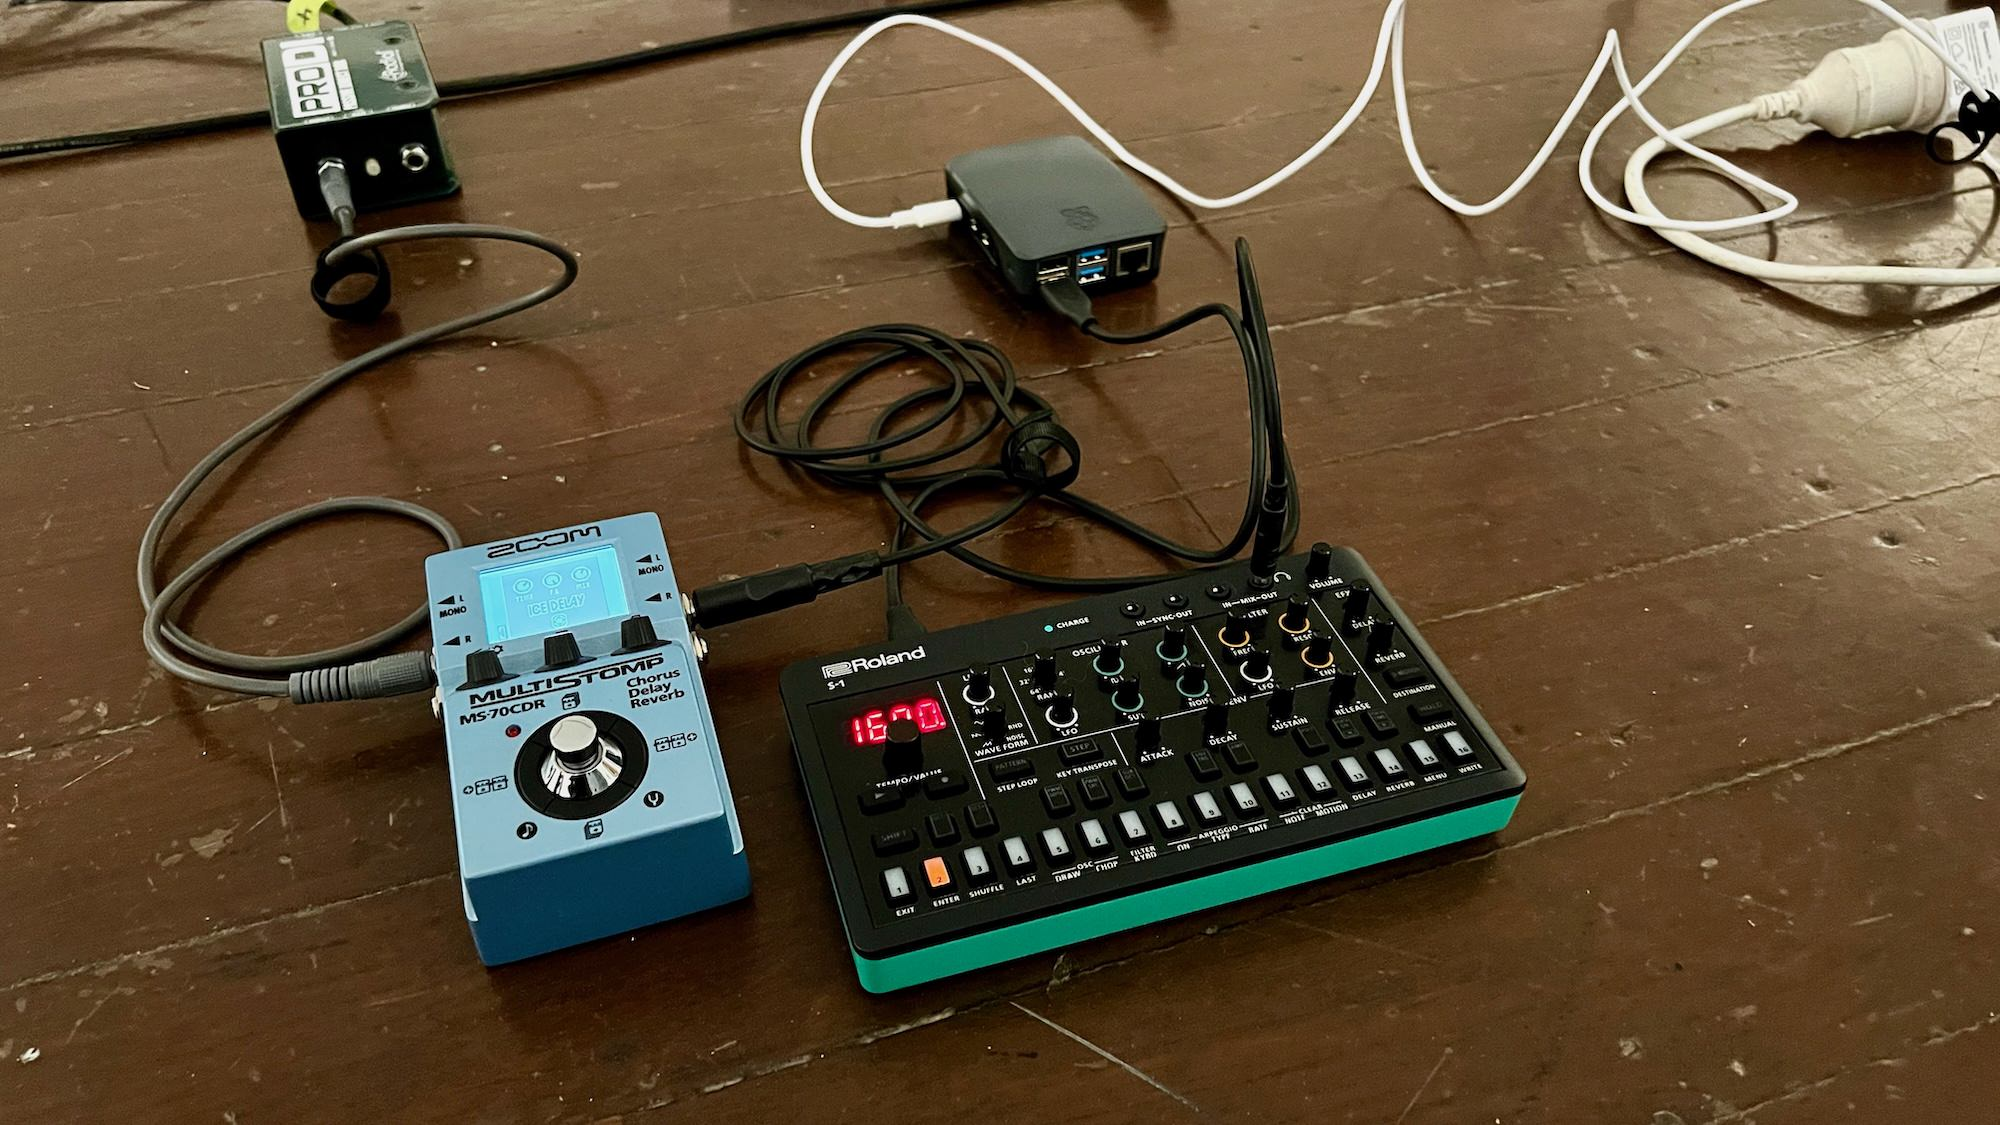
\includegraphics[width=0.8\linewidth]{figures/intelligent-s-1.jpg}
	\caption{A performance setup on the floor with the Roland S-1 synthesiser, Zoom effects pedal, and IMPSYpi running on a Raspberry Pi 4. This setup was used in a free-improvisation ensemble with performers on different acoustic and electronic instruments.}
	\label{fig:s-1}
\end{figure}

%\subsection{Intelligent DAWs: Ableton Live and Kymatica AUM}


\section{Conclusions and Future Work}\label{conclusions}

Our system has been tested in the context of electronic music improvisation where control over a synthesiser is shared between a human and the GenAI MIDI Plug. Figure \ref{fig:human-ai} and our accompanying video\footnote{\url{https://vimeo.com/911078203}} shows excerpts from an outdoor battery-powered improvisation. In this example, the synthesiser is a Korg Volca FM with note values (pitch and rhythm) controlled by the GenAI MIDI Plug. The musician adjusts parameters on the synthesiser patch including pitch shifting the GenAI MIDI signals by octaves.

The experience so far with this system is positive. The signal from the GenAI MIDI Plug can be contextualised as a more expressive and unpredictable kind of LFO (low frequency oscillator) within a synth setup. As it's modelled on human-sourced data, it noodles, pauses, explores different parts of the output range, stops completely sometimes and starts up again at (perhaps) annoying moments. Although it exhibits some behaviours that could be programmed into a hard-coded signal generator it also has a level of stochasticity and variation that that would be more complicated to construct heuristically. Importantly, the very small size of the system means that it can fit into battery-powered electronic music setups. The price of the system means that potentially more than one could be affordably applied in any one performance.

The intention of this research has been not just to create one GenAI MIDI Plug but to demonstrate the feasibility of this approach to instrument designers who may wish to adapt this idea.
The hardware aspects of our system demonstrate a really simple way of connecting a Raspberry Pi Zero to existing electronic music systems. 
Although the software is effective, the Keras MDN Layer~\cite{keras-mdn-layer} library presently requires the full Tensorflow and TensorFlow-Probability libraries. 
The newer 64-bit Raspberry Pi OS should make it easier to install these, but in our experience we were still using a custom build of Tensorflow\footnote{\url{https://github.com/PINTO0309/Tensorflow-bin}} for the Raspberry Pi which may be intimidating for beginners to install. 
Once the system is running, data generation with the MDRNN is quick; however, the process of booting, loading Tensorflow, and starting generation takes around 90 seconds. 
There may be potential to port this system to use lighter libraries (e.g., Tensorflow-Lite) that may load more quickly from boot and could also improve the installation experience for instrument designers.

This work has introduced a minimal approach to creating an intelligent musical instrument, the GenAI MIDI Plug. This research aims to address gaps in creative practice and interaction that have been identified in NIME applications of generative AI. While enabling artist-led data collection and training may support a small-data approach, cheap minimal battery-powered AI music controllers could encourage a greater range of experimentation and prototyping among the wider music community.


\bibliographystyle{ACM-Reference-Format}
\bibliography{references} 

\end{document}
